\chapter{Aufbau}
Der Quellcode wurde in folgende Bereiche strukturiert:

\section{Komponenten}
Der \emph{components}-Ordner beinhaltet alle definierten Angular-Komponenten.
Dabei wurde darauf geachtet das diese möglichst modular und einfach gehalten wurden.
Durch den Einsatz von \emph{ngxs} konnte die Fehlerbehandlung und die Geschäftslogik einfach in entsprechende \emph{state}-Services ausgelagert werden.

\section{Modelle}
Der \emph{dtos}-Ordner beinhaltet die Modeldefinitionen von Daten die von der \emph{Hurace.Api} abgefragt werden.
Die Abkürzung \emph{dto} steht dabei für \emph{DataTransferObject}.
Der \emph{enums}- bzw. \emph{models}-Ordner beinhaltet zusätzliche Modeldefinitionen und Enumerationen.

\section{Hurace.Api Dienste}
Der \emph{services}-Ordner beinhaltet Dienste zum Abfragen von Daten der \emph{Hurace.Api}.
Die \emph{LiveService}-Klasse, die als Singleton in der Webanwendung gestartet wird, kümmert sich um die \emph{SinglaR}-Verbindung zum \emph{Hurace.Api}-Server.

\section{Zustandsverwaltung}
Die Zustandsverwaltung der Webanwendung wurde mit der externen Bibliothek \emph{ngxs} gelöst.
Im \emph{actions}-Ordner werden alle Aktionen definiert die den Applikationszustand verändern können.
Aktionen sind als einfache Klassen abgebildet, wie in-\cref{lst:SkierActions} zu sehen.

\begin{lstlisting}[caption={Definieren einer Aktion}, label=lst:SkierActions]
export class GetAllSkiers {
    static readonly type = '[Skier] GetAll';
}
\end{lstlisting}

Eine Aktion kann anschließend über den \emph{store}-Service, der von \emph{ngxs} bereitgestellt wird, in einer Angular-Komponente (\zB SkierListComponent) ausgelöst werden (\cref{lst:DispatchAction}).

\begin{lstlisting}[caption={Auslösen einer Skier-Aktion}, label=lst:DispatchAction]
constructor(private store: Store) { }
ngOnInit() {
    this.store.dispatch(new GetAllSkiers());
}
\end{lstlisting}

Die Services im \emph{states}-Ordner behandeln die ausgelösten Ereignisse und können einen definierten Applikationszustand \emph{initialState} über die \emph{context.patchState}-Methode verändern (\cref{lst:SkierState}).
Die \emph{@Action}-Annotation wird von \emph{ngxs} bereitgestellt und verbindet die Aktion mit der Behandlungsmethode.
Die Methode \emph{skierService.getAll()} lädt alle SkirennläuferInnen über die \emph{Hurace.Api}.

\begin{lstlisting}[caption={Behandeln einer Skier-Aktion}, label=lst:SkierState]
const initialState: SkierStateModel = {
    all: empty(),
    selected: empty()
};

@Action(GetAllSkiers)
getAllSkier(context: Context) {
    context.patchState({ all: loading() });

    return this.skierService.getAll().pipe(
        tap(skiers => context.patchState({ all: data(skiers) })),
        catchError(e => context.patchState({ all: error(e) }))
    );
}
\end{lstlisting}

Damit die Angular-Komponente, die das Ereignis ausgelöst hat die Änderungen (Liste an SkirennläuferInnen) mitbekommt kann auf den Applikationszustand gehört werden (\cref{lst:subscribe}).

\begin{lstlisting}[caption={Hören auf Zustandsänderungen}, label=lst:subscribe]
constructor(private store: Store) {
    store.select(s => s.skier.all)
        .subscribe(skiers => {
            // skier list changed
        });
}
\end{lstlisting}

Über die Browsererweiterung \emph{Redux DevTools} können außerdem alle Zustandsänderungen der jeweiligen Ereignisse verfolgt werden.
Voraussetzung ist die Registrierung der \emph{Redux DevTools} im Angular-Module mittels \emph{NgxsReduxDevtoolsPluginModule.forRoot()}.
\cref{fig:reduxDevTools} zeigt den Applikationszustand nach Laden eines Skierläufers.
\begin{figure}[H]
    \centering
    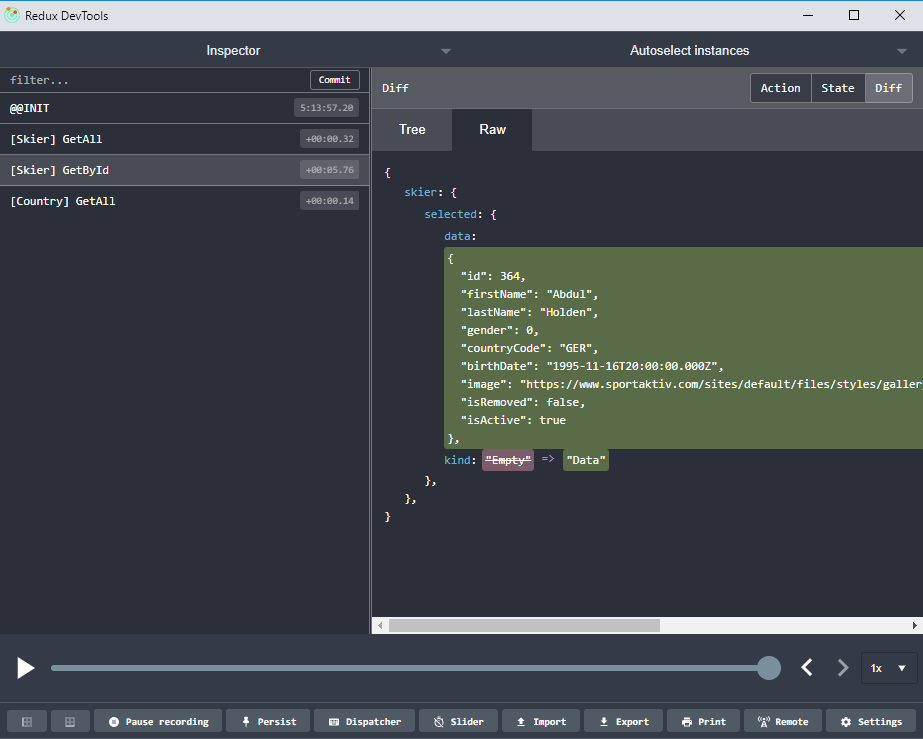
\includegraphics[width=0.9\linewidth]{images/redux-dev-tool}
    \caption{Browsererweiterung Redux DevTools}
\label{fig:reduxDevTools}
\end{figure}
